\documentclass[10pt]{article}
\usepackage{icmlko}

\icmlmeta{IP 파운데이션 월드모델}{231}{죽은 줄 모르고 있었다}{노트 230이 F1 의 nan 을 그냥 넘어간 것을 빚으로 적었다. 열어 보니 기준선이 여덟 도메인에서 죽어 있었고 판정치가 그것을 숨기고 있었다}

\begin{document}

\twocolumn[
\icmlheader

\begin{abstract}
노트 230이 ``F1 프로크루스테스가 이 축 판에서 nan 인데 그냥 넘어갔다''를
빚으로 적었다. 열었다. \textbf{F1 은 아홉 도메인 중 여덟에서 예측이 통째로
NaN 이다} --- 살아 있는 것은 펀딩 80건뿐이다. \textbf{그런데 판
$+$0.1472 를 보고했다.} 축을 더할수록 나빠진다 --- 기본 축에서 넷이 살고,
검색을 얹으면 하나만 남는다. 까닭은 \texttt{rank.pooled} 이 유한 표본
20 미만이거나 예측 분산 0 인 도메인을 \emph{조용히 버리기} 때문이다.
\textbf{그래서 여덟 도메인에서 죽은 정식화도 숫자를 받고, 그 숫자가 아홉
도메인에서 나온 숫자와 같은 눈금에 적힌다.} F1 은 노트 5$\sim$124 의 옛
파이프라인이고 포트폴리오의 기준선이다 --- \textbf{기준선이 오래전부터
죽어 있었고 판정치가 그것을 숨겼다.} F17(무리 전용)은 아예
\texttt{IndexError} 로 터진다. \textbf{분모 가드는 이것을 못 잡는다} ---
분모 가드는 \emph{점수가 있는} 대상을 세는데 죽은 도메인은 애초에 점수가
안 만들어져 분모에서 빠진다. 고쳤다: \texttt{rank.coverage} ·
\texttt{rank.pooled\_cov} 로 \textbf{판정치가 덮음을 같이 들고 다니게}
하고, \textbf{가드 열여섯번째 ``살아있음''} 을 붙였다 --- 자료에 있는
도메인의 80\% 미만에서만 점수가 나면 막는다. F1 이 1/10 (표본 80)로
깨지고 F21 · F23 이 9/10 (2,565)로 통과한다. \textbf{노트 220이 같은
모양을 축 무리 쪽에서 봤는데}(``기타 단독 $+$0.5037'' 이 게임 혼자
값이었다) \textbf{이번엔 판정치 자체다} --- 그 표는 내가 한 번 만든
것이지만 판 $\rho$ 는 이 프로젝트의 순위 기준이다.
\end{abstract}
]

\begin{figure*}[t]
\centering
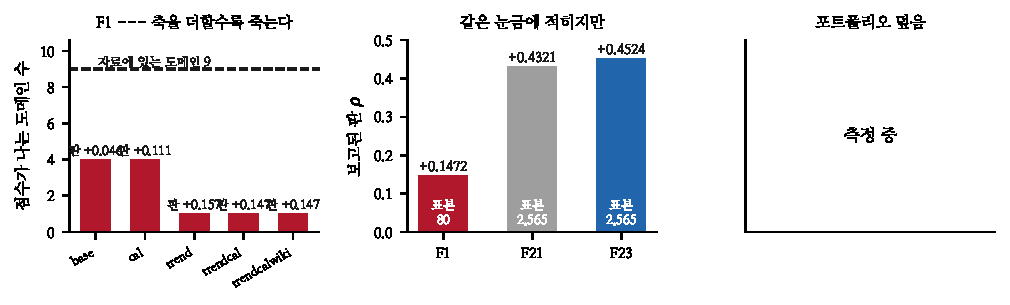
\includegraphics[width=\textwidth]{figs/alive.pdf}
\caption{왼쪽 --- 축을 더할수록 F1 이 죽는다. 가운데 --- 같은 눈금에
적히지만 표본이 80 대 2,565 다. 오른쪽 --- 포트폴리오 덮음.}
\end{figure*}

\section{기준선이 죽어 있었다}

\begin{table}[t]
\centering\tsize
\caption{F1 프로크루스테스. 축 판마다 점수가 나는 도메인 수(자료에는 9).}
\begin{tabular}{lrrl}
\toprule
축 판 & 살아있음 & 보고한 판 & \\
\midrule
base & 4 & $+$.0461 & \\
cal & 4 & $+$.1105 & \\
trend & \textbf{1} & $+$.1566 & \\
trendcal & \textbf{1} & $+$.1472 & \\
\textbf{trendcalwiki} & \textbf{1} & \textbf{$+$.1472} & 펀딩 80건 \\
\bottomrule
\end{tabular}
\end{table}

\claimx{\textbf{축을 더할수록 죽는다} --- 기본 축에서 넷이 살고 검색을
얹으면 하나만 남는다. \textbf{그런데 보고하는 판은 오히려 올라간다}
($+$0.0461 $\to$ $+$0.1472).}{살아남은 도메인이 펀딩 하나이고 펀딩이
$+$0.1472 이기 때문이다 --- \textbf{판이 올라간 것이 아니라 분모가
줄어든 것이다.}}

\claimx{\textbf{F1 은 노트 5$\sim$124 의 옛 파이프라인이고 포트폴리오의
기준선이다.} 기준선이 오래전부터 죽어 있었다.}{F17(무리 전용)은 아예
\texttt{IndexError} 로 터진다. \textbf{포트폴리오가 열아홉인 줄 알았는데
둘은 없는 것이었다.}}

\section{판정치가 숨겼다}

\claimx{\texttt{rank.pooled} 은 유한 표본이 20 미만이거나 예측 분산이
0 인 도메인을 \emph{조용히 버린다}. \textbf{여덟에서 죽은 정식화도 숫자를
받고, 그 숫자가 아홉에서 나온 숫자와 같은 눈금에 적힌다.}}{\textbf{분모
가드는 못 잡는다} --- 분모 가드는 \emph{점수가 있는} 대상을 세는데 죽은
도메인은 애초에 점수가 안 만들어져 분모에서 빠진다. \textbf{가드가
보는 곳에 이미 없다.}}

\begin{table}[t]
\centering\tsize
\caption{같은 눈금에 적히는 세 수.}
\begin{tabular}{lrrr}
\toprule
& 판 $\rho$ & 도메인 & 표본 \\
\midrule
\textbf{F1} & \textbf{$+$.1472} & \textbf{1/9} & \textbf{80} \\
F21 & $+$.4321 & 9/9 & 2{,}565 \\
F23 & $+$.4524 & 9/9 & 2{,}565 \\
\bottomrule
\end{tabular}
\end{table}

\claimx{\textbf{노트 220이 같은 모양을 축 무리 쪽에서 봤다} --- ``기타
단독 $+$0.5037'' 이 판 전체($+$0.4396)를 넘었는데 게임 혼자 값이었다.
\textbf{이번엔 판정치 자체다.}}{그 표는 내가 한 번 만든 것이라 한 번 보고
말지만 \textbf{판 $\rho$ 는 이 프로젝트의 순위 기준이다} --- 같은 병이
훨씬 나쁜 자리에 있었다.}

\section{고침}

\claimx{\textbf{\texttt{rank.coverage} · \texttt{pooled\_cov}} --- 판정치가
덮음을 같이 들고 다니게 했다. 떼어 놓으면 또 이 일이 난다.}{\textbf{가드
열여섯번째 ``살아있음''} --- 자료에 있는 도메인의 80\% 미만에서만 점수가
나면 막는다. F1 1/10 깨짐 · F21 9/10 통과 · F23 9/10 통과.}

\claimx{\textbf{이것은 노트 187의 제일 값싼 검사의 사촌이다} --- 거기서는
``판이 넷째 자리까지 안 움직이면 모형에 안 닿은 것''이었고, 여기서는
\textbf{``판이 나오면 살아 있는 것''이 아니다.}}{둘 다 \emph{숫자가
나왔다는 것}을 \emph{작동했다는 것}으로 읽은 데서 온다.}

\begin{table}[t]
\centering\tsize
\caption{남은 것.}
\begin{tabular}{ll}
\toprule
\textbf{F1 을 살릴까} & 기준선이 없으면 견줄 것이 없다 \\
\textbf{F17} & IndexError --- 고칠지 뺄지 \\
옛 노트 & F1 수를 인용한 노트가 몇인가 \\
\bottomrule
\end{tabular}
\end{table}

셋째 줄이 제일 무겁고 값싸다. \textbf{F1 이 언제부터 죽었는지 모른다.}
노트 125 이후 포트폴리오로 돌면서 F1 을 기준선으로 인용한 노트가 여럿이고,
그 인용이 \emph{네 도메인} 값이었는지 \emph{한 도메인} 값이었는지에 따라
그 노트들의 비교가 성립하는지가 갈린다. \textbf{덮음을 안 적었으므로
지금은 알 수 없고, 알아내려면 축 판마다 F1 을 다시 돌려 봐야 한다} ---
이 노트가 그 다섯 칸을 이미 쟀으므로(base 4 · cal 4 · trend 이후 1)
\textbf{어느 노트가 어느 축 판을 썼는지만 대조하면 된다.} 그리고 그것이
이번 사이클의 마지막 교훈이다 --- \textbf{판정치에 덮음을 안 적으면 옛
수치가 무엇이었는지 나중에 복원할 수 없다.}

\end{document}
